\chapter{Dynamic programming I: the method and the classics}\label{ch:dp1}
\index{dynamic programming}\index{memoization}\index{knapsack}\index{LIS}

Dynamic programming is not an algorithm --- it is a bookkeeping
promise: never solve the same subproblem twice. The craft is five
choices in order (state, transition, base case, fill order, answer
location), plus one trap that wrong-answers more submissions than
every other combined: ordered versus unordered counting. After this
chapter you will run the recipe end to end on coins, knapsack, LIS
and grids, and know the two loop orders by heart.

% from-zero:begin
\begin{rulebox}[Before you start]
Chapters~2 and~5. \emph{Recap:} complete search (Chapter~2) can recompute the same sub-problem thousands of times. Dynamic programming is complete search plus a table that remembers answers; you will see this on a problem you have already solved.
\end{rulebox}
\begin{wins}[After this chapter you can]
\begin{itemize}
\item turn a recursive brute force into a table by naming the state and writing the transition;
\item solve coin-change, knapsack, longest-increasing-subsequence and grid-path problems;
\item decide whether a problem wants DP or a greedy;
\item recover the actual solution, not just its value, from a DP table.
\end{itemize}
\end{wins}
\begin{principle}[How to think about this]
Dynamic programming sounds grand but is a modest idea: write the slow recursive solution, notice that it keeps solving the same small problems, and store each answer the first time. The skill is choosing the \emph{state}: the smallest description of where you are that still tells you everything you need about the future. Always say your state and your transition in one plain sentence before you write a line of code.
\end{principle}
% from-zero:end

\section{The same problem twice}\label{sec:memo}
Memoization recurses and caches; tabulation fills a table in
dependency order. They compute the \emph{same set} --- memoization
visits only reachable states (safer when the state space is sparse),
tabulation visits all states in order (safer on recursion depth).

\section{The DP recipe}\label{sec:recipe}
Five lines: (1) \emph{state} --- what identifies a subproblem;
(2) \emph{transition} --- how it reduces; (3) \emph{base case};
(4) \emph{order} --- dependencies before dependents (this is DP on
the subproblem DAG, Figure~\ref{fig:subdag}); (5) \emph{answer} ---
which state(s) to read.
\begin{figure}[ht]\centering
% fig50-subdag.tex -- Figure 11.x: subproblem DAG for min-coin DP, coins {1,3,4}, amount 6.
% fstyle.tex -- shared TikZ styles for the figures of this book (palette from lifeos.sty).
\tikzset{%
  cell/.style={draw=ink, minimum width=7mm, minimum height=6.5mm, inner sep=0pt, font=\footnotesize, fill=white},
  cellh/.style={cell, fill=accentsoft, draw=accent},
  cella/.style={cell, fill=amberbg, draw=amber},
  cellg/.style={cell, fill=goodbg, draw=good},
  cellx/.style={cell, fill=graybg, draw=slate, text=slate},
  vtx/.style={circle, draw=ink, minimum size=6.5mm, inner sep=0pt, font=\footnotesize, fill=white},
  vtxh/.style={vtx, draw=accent, fill=accentsoft},
  vtxa/.style={vtx, draw=amber, fill=amberbg},
  vtxg/.style={vtx, draw=good, fill=goodbg},
  vtxd/.style={vtx, draw=slate, fill=graybg, text=slate},
  lab/.style={font=\footnotesize, text=slate},
  labA/.style={font=\footnotesize, text=accent},
  labM/.style={font=\footnotesize, text=amber},
  idx/.style={font=\tiny, text=slate},
  arr/.style={-{stealth}, thick, ink},
  arrA/.style={-{stealth}, thick, accent},
  arrM/.style={-{stealth}, thick, amber},
  arrG/.style={-{stealth}, thick, good},
  edge/.style={thick, ink},
  edgeA/.style={thick, accent},
  edgeM/.style={thick, amber},
}%
% \cellrow{prefix}{x0}{y}{style}{v0,v1,...}: a row of cells named prefix0, prefix1, ... (pitch 0.75cm)
\providecommand{\cellrow}[5]{\foreach \v [count=\i from 0] in {#5} {\node[#4] (#1\i) at (#2+\i*0.75,#3) {\v};}}%
% \cellidx{prefix}{n}{start}: index labels under cells prefix0 .. prefix(n-1)
\providecommand{\cellidx}[3]{\foreach \i in {0,...,\numexpr#2-1\relax} {\node[idx, below=0pt of #1\i] {\the\numexpr\i+#3\relax};}}%
% \fitfig{<tikzpicture>}: shrink the picture to \linewidth only when it would overflow.
\ifdefined\fitbox\else\newsavebox{\fitbox}\fi%
\providecommand{\fitfig}[1]{\sbox{\fitbox}{#1}\ifdim\wd\fitbox>\linewidth\resizebox{\linewidth}{!}{\usebox{\fitbox}}\else\usebox{\fitbox}\fi}%

\begin{tikzpicture}[font=\footnotesize]
\foreach \i in {0,...,6} \node[vtx, minimum size=7mm] (d\i) at (\i*1.6,0) {\i};
\foreach \i in {1,...,6} \draw[arr, shorten >=1pt, shorten <=1pt, bend left=45] (d\i) to (d\the\numexpr\i-1\relax);
\foreach \i in {3,...,6} \draw[arrA, shorten >=1pt, shorten <=1pt, bend right=40] (d\i) to (d\the\numexpr\i-3\relax);
\foreach \i in {4,...,6} \draw[arrM, shorten >=1pt, shorten <=1pt, bend right=55, looseness=1.1] (d\i) to (d\the\numexpr\i-4\relax);
\node[lab, anchor=west, align=left] at (0,-3.4) {node $x$: ``fewest coins for amount $x$''; edge $x\to x-c$: ``last coin was $c$''};
\node[lab, anchor=west, align=left] at (0,-4.0) {coin $1$ black (below), coins $3$ blue and $4$ amber (above); fill order $0,1,\dots,6$ is a topological order};
\end{tikzpicture}

\caption{The subproblem DAG for coin DP. Notice ``topological order''
is literally a fill order --- that is what DP is.}
\label{fig:subdag}
\end{figure}

\section{Coin problems}\label{sec:coins}\index{coin DP}
Minimising coins is minimisation (min over last coin); counting ways
is summation --- and the summation splits into two different
problems by loop order.
\begin{example}[CSES \emph{Minimizing Coins}]\label{ex:coins}
Fewest coins to make $x$.
\par\smallskip
\textbf{Strategy.} State = amount; transition = min over last coin
used. Top-down and bottom-up compute the same states.
\par\smallskip
\begin{solution}
\lstinputlisting{code/minimizing_coins.cpp}
Real output (CSES sample):
\begin{lstlisting}[numbers=none]
3
\end{lstlisting}
\end{solution}
\end{example}
\begin{example}[CSES \emph{Dice Combinations} \textrightarrow\
\emph{Coin Combinations I vs II}]\label{ex:combos}
Ways to sum to $x$: I counts ordered sequences, II unordered
multisets.
\par\smallskip
\textbf{Strategy.} Same table, different nesting: sum-outer counts
permutations separately (ordered); coin-outer fixes each coin's
count before the next (unordered). Swap the loops, swap the answer.
\par\smallskip
\begin{solution}
\lstinputlisting{code/coin_combos.cpp}
Real output (CSES sample, I then II):
\begin{lstlisting}[numbers=none]
8 3
\end{lstlisting}
\end{solution}
\end{example}
\begin{figure}[ht]\centering
\begin{tikzpicture}[font=\footnotesize]
\begin{scope}
\node[font=\tiny] at (0.9,0.9) {sum-outer (ordered)};
\node[font=\tiny] at (0.9,0.4) {$\{2,3\}$ and $\{3,2\}$ both counted};
\node[font=\tiny,draw=slate] at (0.9,-0.2) {answer 8};
\end{scope}
\begin{scope}[xshift=5cm]
\node[font=\tiny] at (0.9,0.9) {coin-outer (unordered)};
\node[font=\tiny] at (0.9,0.4) {$\{2,3\}$ counted once};
\node[font=\tiny,draw=slate] at (0.9,-0.2) {answer 3};
\end{scope}
\node[font=\tiny,align=center] at (2.5,-1.3) {same recurrence, different loop order};
\end{tikzpicture}

\caption{The ordered/unordered split. Notice both use the identical
recurrence --- the loop order \emph{is} the difference.}
\label{fig:ordbug}
\end{figure}

\section{Knapsack}\label{sec:knap}\index{knapsack}
0/1 knapsack: each item at most once --- the inner capacity loop must
run \emph{descending}, or item $i$ reuses itself and you have solved
the unbounded problem. Unbounded is the ascending twin.
Reconstruction walks the table backwards.
\begin{example}[CSES \emph{Book Shop}]\label{ex:shop}
Max pages within budget.
\par\smallskip
\textbf{Strategy.} $\texttt{dp}[i][x]$ = best using items $1..i$;
descend capacity so item $i$ appears at most once.
\par\smallskip
\begin{solution}
\lstinputlisting{code/book_shop.cpp}
Real output (CSES sample; second line is the reconstructed
take-table --- books 1 and 3, weight $4+5\le 10$, value $5+8=13$):
\begin{lstlisting}[numbers=none]
13
1 3
\end{lstlisting}
\end{solution}
\end{example}
\begin{figure}[ht]\centering
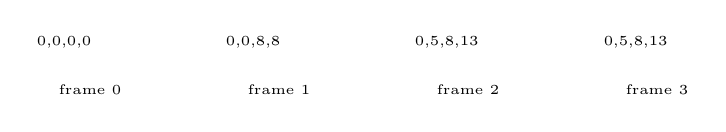
\begin{tikzpicture}[font=\tiny]
\foreach \i/\c in {0/{0,0,0,0},1/{0,0,8,8},2/{0,5,8,13},3/{0,5,8,13}}{
  \begin{scope}[xshift=\i*2.4cm]
    \foreach \r/\row in {0/\c}
      \node[anchor=west] at (0,0) {\row};
    \node at (0.8,-0.6) {frame \i};
  \end{scope}}
\end{tikzpicture}

\caption{Book Shop's table filling. Notice each frame only reads the
previous row --- that dependency shape is what licenses the
one-array version.}
\label{fig:dpfill}
\end{figure}

\section{LIS in \texorpdfstring{$O(n\log n)$}{O(n log n)}}\label{sec:lis}\index{LIS}
Keep $L[i]$ = smallest possible tail of an increasing subsequence of
length $i{+}1$. Three lemmas (USACO-Guide style): $L$ is always
sorted; each read $x$ replaces $\texttt{lower\_bound}(x)$, never
lengthening unless it appends; the answer is $|L|$.
\begin{lstlisting}[language=C++,caption={\texttt{lis.h}: the
7-line core.},label={lst:lis}]
\end{lstlisting}
\lstinputlisting{code/lis.h}
\begin{example}[CSES \emph{Increasing Subsequence}]\label{ex:lis}
Longest strictly increasing subsequence.
\par\smallskip
\textbf{Strategy.} The $O(n^2)$ is obvious; the tableau version is
the same answers in $O(n\log n)$.
\par\smallskip
\begin{solution}
\lstinputlisting{code/increasing_subseq.cpp}
Real output (CSES sample):
\begin{lstlisting}[numbers=none]
4
\end{lstlisting}
\end{solution}
\end{example}
\begin{figure}[ht]\centering
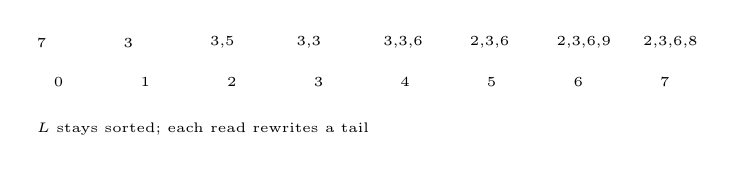
\begin{tikzpicture}[font=\tiny]
\foreach \i/\L in {0/{7},1/{3},2/{3,5},3/{3,3},4/{3,3,6},5/{2,3,6},6/{2,3,6,9},7/{2,3,6,8}}{
  \node[anchor=west] at (\i*1.1,0) {\L};
  \node at (\i*1.1+0.4,-0.5) {\i};
}
\node[anchor=west] at (0,-1.1) {$L$ stays sorted; each read rewrites a tail};
\end{tikzpicture}

\caption{The patience array evolving. Notice $L$'s length is the
answer --- its entries are only potential tails.}
\label{fig:patience}
\end{figure}

\section{Grid DP}\label{sec:griddp}\index{grid DP}
Paths through a grid pull from left and above; obstacles are just
zeros. In-place filling works because each cell only reads already-
computed cells.
\begin{example}[CSES \emph{Grid Paths I}]\label{ex:grid}
Paths through a grid with traps.
\par\smallskip
\textbf{Strategy.} dp[r][c] = left + below; trap cells contribute 0.
\par\smallskip
\begin{solution}
\lstinputlisting{code/grid_paths.cpp}
Real output (CSES sample):
\begin{lstlisting}[numbers=none]
3
\end{lstlisting}
\end{solution}
\end{example}
\begin{figure}[ht]\centering
\begin{tikzpicture}[font=\footnotesize,x=0.5cm,y=0.5cm]
\foreach \x in {0,...,3} \foreach \y in {0,...,3}
  \draw[slate!60] (\x,\y) rectangle +(1,1);
\fill[accentsoft] (2,2) rectangle +(1,1);
\draw[-{stealth},amber,thick] (1.5,2.5)--(2.5,2.5);
\draw[-{stealth},amber,thick] (2.5,1.5)--(2.5,2.5);
\node[font=\tiny] at (2,-0.7) {cell (i,j) pulls from left and below};
\end{tikzpicture}

\caption{Grid dependencies. Notice the two-source pull is why a
single pass suffices --- every cell's inputs are computed earlier.}
\label{fig:griddep}
\end{figure}

\section{Push vs pull}\label{sec:pushpull}
Pull: each state reads its predecessors. Push: each state updates its
successors. Same recurrence, different direction --- pull is usually
clearer; push wins when the frontier is sparse.

\begin{exercise}[easy]\label{exr:state}
State for ``largest sum ending exactly at index $i$'' vs ``largest
sum anywhere in $1..i$'' --- which is which, and why can't they swap?
\end{exercise}
\begin{exercise}[medium]\label{exr:ord}
Coins $\{1,2\}$, $x=3$: enumerate the ordered and unordered counts
and explain the missing summands.
\end{exercise}
\begin{exercise}[medium]\label{exr:dir}
An ascending inner loop in 0/1 knapsack is a \emph{different}
problem. Name it and explain the single direction change.
\end{exercise}
\begin{exercise}[medium]\label{exr:predbug}
Predict the output of coin-outer counting if the answer table
printed is not the final cell but a sum over all cells --- what goes
wrong?
\end{exercise}

\section{Chapter summary}
\begin{table}[ht]\centering
{\small
\begin{tabularx}{\linewidth}{@{}lYYY@{}}
\toprule
\tablehead\thead{Problem} & \thead{State} & \thead{Transition} & \thead{Trap}\\
\midrule
min coins & amount & min over last coin & INF guard\\
count ways (ord) & amount & sum-outer loops & order counted\\
count ways (unord) & amount & coin-outer loops & order collapsed\\
0/1 knapsack & (item, cap) & descending cap & self-reuse\\
LIS & tail min & lower\_bound & strict vs non\\
grid paths & (r,c) & left + below & obstacles = 0\\
\bottomrule
\end{tabularx}}
\caption{Five states, five transitions --- and the loop order that
changes the answer, not the code.}
\label{tab:dp}
\end{table}

\section{Common mistakes}
\index{common mistakes}
\begin{itemize}
\item \textbf{Ordered-vs-unordered swap.} The single most common
wrong answer: fix the loop nesting to the semantics asked.
\item \textbf{Ascending capacity on 0/1 knapsack.} Item reuse slips
in silently --- descend, or use two rows.
\item \textbf{INF arithmetic.} \texttt{min + 1} on an unreachable
state overflows --- guard with a sentinel comparison.
\item \textbf{Iterating coins inside on unbounded with reuse across
calls.} Recompute per case; shared tables bleed answers.
\item \textbf{LIS strictness.} \texttt{lower\_bound} for strict,
\texttt{upper\_bound} for non-decreasing --- swapping them silently
changes the problem.
\end{itemize}

\section{Additional exercises}
\begin{exercise}[easy] CSES \emph{Coin Combinations I/II}. \end{exercise}
\begin{exercise}[easy] CSES \emph{Removing Digits} --- greedy-ish DP. \end{exercise}
\begin{exercise}[easy] CSES \emph{Money Sums} --- reachable sums. \end{exercise}
\begin{exercise}[easy] USACO-G \emph{Fruit Feast} --- knapsack variant. \end{exercise}
\begin{exercise}[medium] CSES \emph{Array Description} --- bounded DP. \end{exercise}
\begin{exercise}[medium] CSES \emph{Two Sets II} --- subset-sum DP. \end{exercise}
\begin{exercise}[medium] CSES \emph{Rectangle Cutting} --- cuts DP. \end{exercise}
\begin{exercise}[medium] USACO-G \emph{Hoof, Paper, Scissors} --- prefix-state DP. \end{exercise}
\begin{exercise}[medium] USACO-G \emph{Time is Mooney} --- time-expanded DP. \end{exercise}
\begin{exercise}[medium] USACO-G \emph{Teamwork} --- group-sum DP. \end{exercise}
\begin{exercise}[medium] CSES \emph{Grid Paths} (DP set) --- grid DP over reachable cells. \end{exercise}
\begin{exercise}[medium] CSES \emph{Counting Towers} --- state-pair recurrence; find the two states yourself. \end{exercise}
\begin{exercise}[hard] CSES \emph{Projects} --- weighted intervals DP. \end{exercise}
\begin{exercise}[hard] USACO-G \emph{Snakes} --- herds DP. \end{exercise}
\begin{exercise}[hard] USACO-G \emph{Talent Show} --- ratio DP. \end{exercise}

\chapternotes
The memo/tabulation framing and the ordered-unordered centerpiece
follow Laaksonen~\cite{laaksonen2024} and Sannemo~\cite{sannemo2025};
the patience-tableau three-lemma LIS is the USACO Guide's
presentation~\cite{usacoguide}; knapsack loop-direction and grid DP
are standard in cp-algorithms~\cite{cpalgorithms} and
Halim~\cite{halimcp4}; archive problems are official
CSES/USACO~\cite{cses}.

\section*{Further reading}
\begin{itemize}
\item USACO Guide, ``Introduction to DP'' (intermediate) --- the state/transition
method of \S\ref{sec:recipe} with Gold-level problems. \newline\url{https://usaco.guide/gold/intro-dp}
\item USACO Guide, ``Knapsack DP'' (intermediate) --- \S\ref{sec:knap} extended
to its classic variants. \newline\url{https://usaco.guide/gold/knapsack}
\item USACO Guide, ``Longest Increasing Subsequence'' (intermediate) --- \S\ref{sec:lis} including the
$O(n\log n)$ patience form. \newline\url{https://usaco.guide/gold/lis}
\item cp-algorithms, ``Introduction to Dynamic Programming''
(reference).
--- memoization-vs-tabulation of \S\ref{sec:memo}. \newline\url{https://cp-algorithms.com/dynamic_programming/intro-to-dp.html}
\item CSES 1633 \emph{Dice Combinations} and 1634 \emph{Minimizing
Coins} (practice) ---
\ref{ex:combos}/\ref{ex:coins} verbatim. \newline\url{https://cses.fi/problemset/task/1633}
\item CSES 1158 \emph{Book Shop} and 1145 \emph{Increasing
Subsequence} (practice).
--- the chapter's two flagship submissions. \newline\url{https://cses.fi/problemset/task/1158}\end{itemize}

\begin{rulebox}[Watch instead]
\smallskip\noindent\textbf{Best first.}
``15. Dynamic Programming, Part 1: SRTBOT, Fib, DAGs, Bowling'' ---
MIT OpenCourseWare, 57 min ---
\url{https://youtu.be/r4-cftqTcdI}. The
subproblem/recurrence/topological/bottom-up recipe of
\S\ref{sec:recipe}---\S\ref{sec:memo}; OCW names it ``SRTBOT'', the
book names the same five questions without the acronym.
\smallskip\noindent
``16. Dynamic Programming, Part 2: LCS, LIS, Coins'' --- MIT
OpenCourseWare, 59 min ---
\url{https://youtu.be/KLBCUx1is2c}. The coin and LIS
recurrences of \S\ref{sec:coins} and \S\ref{sec:lis} derived on the
board; same formulation, same memo/table duality. Access date
2026-10-10.
\end{rulebox}
